\documentclass[12pt]{article}

\usepackage[a4paper, margin=0.70in]{geometry}
\usepackage{newtxtext,newtxmath}
\usepackage{graphicx}
\usepackage{amsmath}
\usepackage{float}
\usepackage{listings}
\usepackage[colorlinks=false, pdfborder={0 0 0}]{hyperref}
\usepackage{color}
\usepackage{authblk}
\usepackage{caption}
\usepackage{enumitem}
\usepackage{xcolor}
\usepackage{booktabs}
\usepackage{tikz}
\usepackage{ragged2e}

\lstset{
  frame=single,
  breaklines=true,
  showstringspaces=false,
  breakatwhitespace=true,
  basicstyle=\ttfamily\small,
  stringstyle=\color{orange},
  backgroundcolor=\color{gray!10},
  commentstyle=\color{gray}\itshape,
  keywordstyle=\color{blue}\bfseries,
}

\title{
  \Huge \textbf{Sentiment Analysis using Feed-Forward and LSTM Models}
}

\author[1]{Satish Jhanwer}

\affil[1]{Roll No: G24AIT009}

\date{\today}

\begin{document}
\justifying

\begin{titlepage}
  \centering
  
\includegraphics[width=0.2\textwidth]{images/logo.png}\par\vspace{1cm}

  {\Huge \bfseries Cyber Security \par}
  \vspace{0.5cm}
  {\Large Assignment 2: CIC-Darknet2020 Traffic Classification \par}
  \vspace{1cm}

  \begin{tabular}{rl}
    Satish Jhanwer & (G24AIT009) \\
  \end{tabular}

  \vfill

  Indian Institute of Technology Jodhpur \\
  \vspace{0.5cm}
  Date: \today

\end{titlepage}

\newpage

\begin{abstract}
  This report presents the preprocessing, modeling, and evaluation of network traffic data from the CIC-Darknet2020 dataset. Two classification tasks are considered: \texttt{Label} (Non-Tor, NonVPN, VPN, Tor) and \texttt{Label.1} (application-level categories such as P2P, Browsing, etc.). HistGradientBoosting classifiers were trained, tuned, and evaluated using metrics including accuracy, log-loss, ROC-AUC, and confusion matrices. Visualizations using PCA, t-SNE, and ROC curves support the analysis.
\end{abstract}

\newpage

\tableofcontents
\listoffigures

\newpage

\section{Introduction}
The CIC-Darknet2020 dataset comprises network flow features labeled by traffic type and application. This assignment aims to build and evaluate machine-learning classifiers to distinguish between encrypted/anonymized traffic (e.g., Tor, VPN) and to identify specific application protocols.


\section{Dataset and Preprocessing}
\subsection{Data Loading}
The raw CSV contains 141,530 flows with 85 columns. After dropping non-numeric fields (Flow ID, IP addresses, timestamps) and removing malformed rows, the feature matrix has 141,481 samples and 79 numeric attributes.

\subsection{Exploratory Analysis}
Figure~\ref{fig:pca} shows a PCA projection of all flows, and Figure~\ref{fig:tsne} presents a t-SNE embedding of a 5k-sample subset.

\begin{figure}[H]
  \centering
  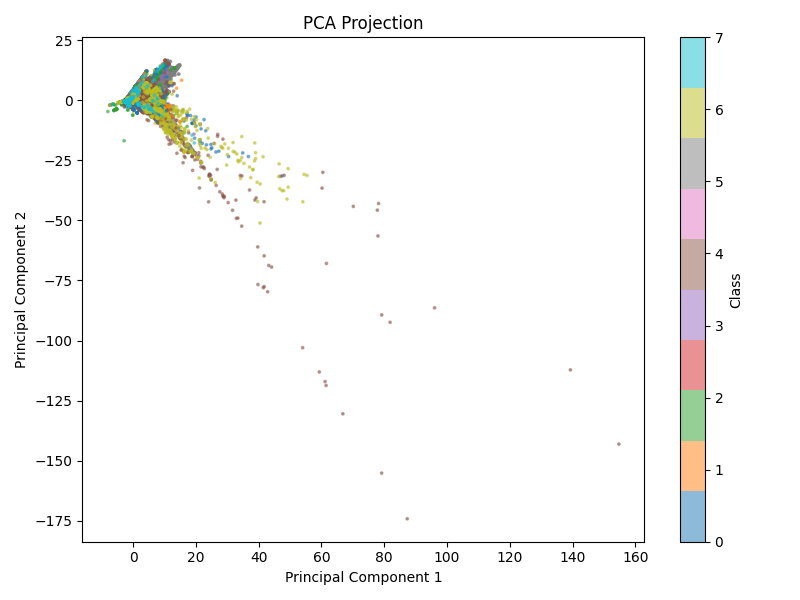
\includegraphics[width=0.8\textwidth]{images/pca_scatter.png}
  \caption{PCA scatter plot of scaled features.}
  \label{fig:pca}
\end{figure}

\begin{figure}[H]
  \centering
  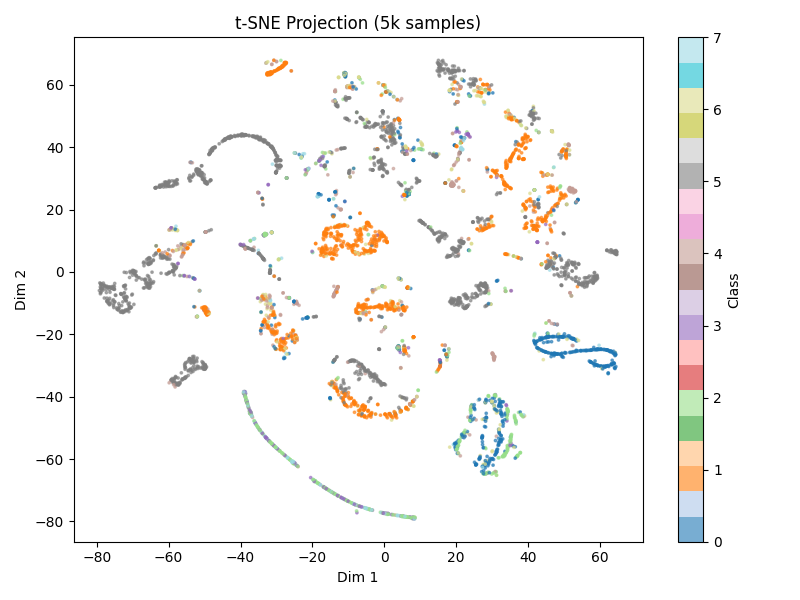
\includegraphics[width=0.8\textwidth]{images/tsne_scatter.png}
  \caption{t-SNE embedding (5k samples).}
  \label{fig:tsne}
\end{figure}

\section{Methodology}
A standard pipeline was implemented:
\begin{enumerate}
  \item Feature scaling via \texttt{StandardScaler}.
  \item Train/validation/test split (68\%/12\%/20\%), stratified by labels.
  \item Hyperparameter tuning of \texttt{HistGradientBoostingClassifier} using \texttt{GridSearchCV} over learning rates \{0.05,0.1,0.2\}, max iterations \{100,200\}, and max depth \{None,10\}.
  \item Evaluation metrics: accuracy, log-loss, ROC-AUC (one-vs-rest), confusion matrix, and classification report.
\end{enumerate}

\section{Results}

\subsection{Task 1: \texttt{Label} Classification}
Grid search selected \texttt{learning\_rate=0.05}, \texttt{max\_depth=None}, \texttt{max\_iter=200}. Validation and test performances:
\begin{itemize}
  \item Validation log-loss: 0.0374
  \item Validation accuracy: 98.66\%
  \item Validation ROC-AUC: 0.9975
  \item Test accuracy: 98.67\%
  \item Test log-loss: 0.0401
  \item Test ROC-AUC: 0.9960
\end{itemize}

Figure~\ref{fig:cm_label} and Figure~\ref{fig:roc_label} illustrate confusion and ROC curves.

\begin{figure}[H]
  \centering
  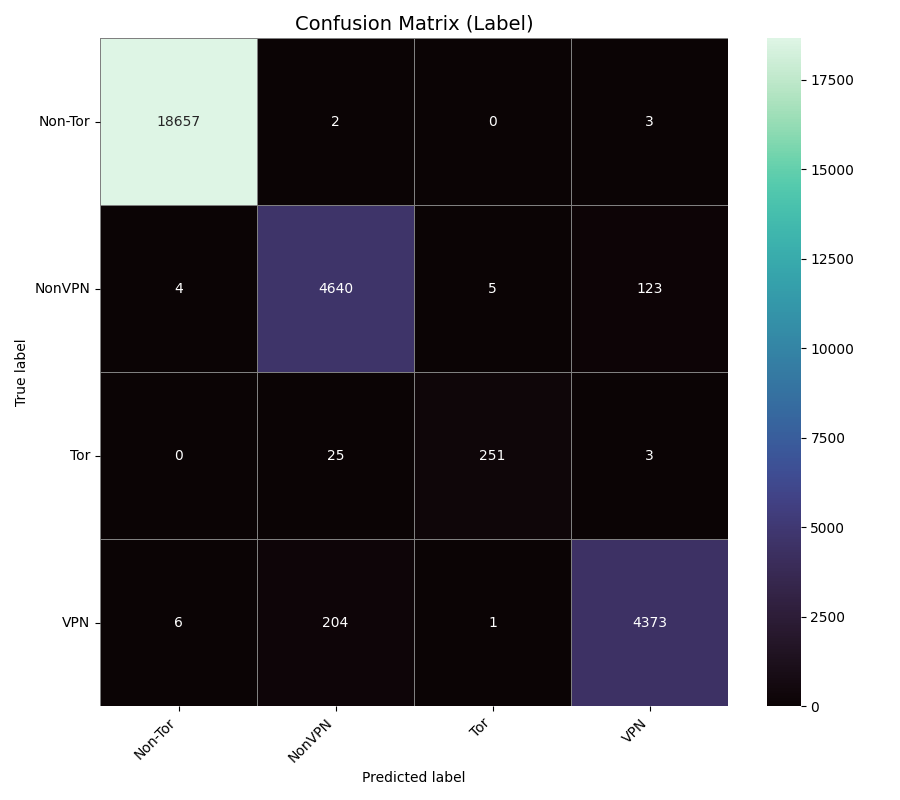
\includegraphics[width=0.8\textwidth]{images/cm_Label.png}
  \caption{Confusion matrix for \texttt{Label} classification.}
  \label{fig:cm_label}
\end{figure}

\begin{figure}[H]
  \centering
  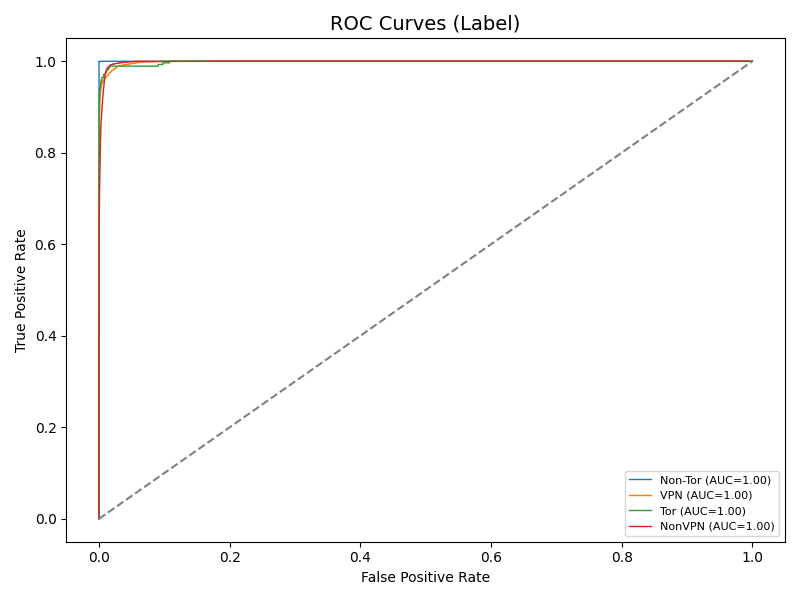
\includegraphics[width=0.8\textwidth]{images/roc_Label.png}
  \caption{ROC curves (one-vs-rest) for \texttt{Label}.}
  \label{fig:roc_label}
\end{figure}

Classification report shows near-perfect precision/recall across all four classes, with minor confusion between NonVPN and VPN flows.

\subsection{Task 2: \texttt{Label.1} Classification}
Best hyperparameter: \texttt{learning\_rate=0.1}, \texttt{max\_depth=None}, \texttt{max\_iter=200}. Metrics:
\begin{itemize}
  \item Validation log-loss: 0.2012
  \item Validation accuracy: 91.57\%
  \item Validation ROC-AUC: 0.9853
  \item Test accuracy: 91.49\%
  \item Test log-loss: 0.1981
  \item Test ROC-AUC: 0.9853
\end{itemize}

\begin{figure}[H]
  \centering
  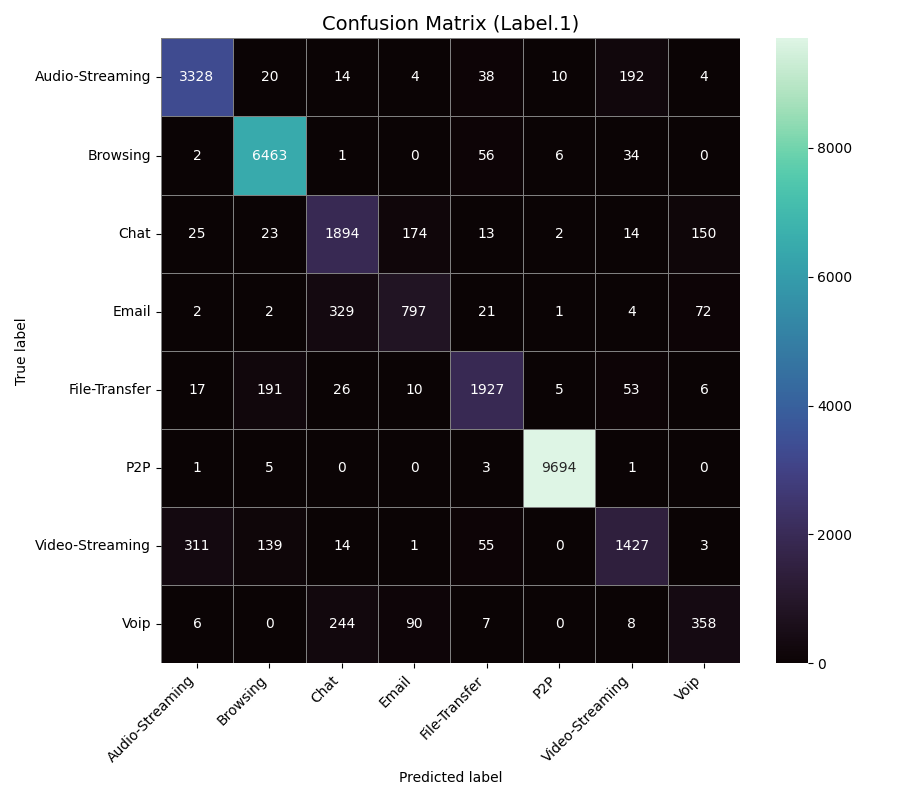
\includegraphics[width=0.8\textwidth]{images/cm_Label.1.png}
  \caption{Confusion matrix for \texttt{Label.1} classification.}
  \label{fig:cm_label1}
\end{figure}

\begin{figure}[H]
  \centering
  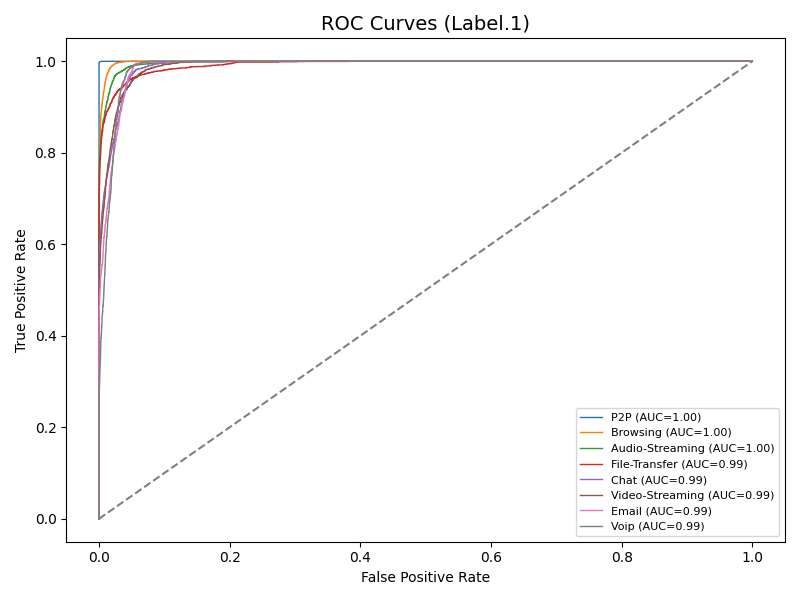
\includegraphics[width=0.8\textwidth]{images/roc_Label.1.png}
  \caption{ROC curves (one-vs-rest) for \texttt{Label.1}.}
  \label{fig:roc_label1}
\end{figure}
The classifier performs well on majority classes such as P2P and Browsing, with recall above 98\%. Classes with fewer samples (e.g., Voip) still show lower recall (50\%) and f1-scores, indicating remaining challenges with class imbalance. The overall accuracy of 91.49\% and ROC-AUC of 0.9853 suggest strong discriminative ability, albeit with room to improve rare-category performance.

\section{Discussion}
The first task demonstrates that HistGradientBoosting easily separates encrypted/anonymized traffic with almost no errors. The second task's lower accuracy (\~90\%) stems from class imbalance and subtle feature overlap between application protocols. Potential improvements:
\begin{itemize}
  \item Merge or normalize duplicate label names (e.g., File-Transfer variants).
  \item Apply SMOTE or class-weight adjustments for rare classes.
  \item Feature engineering: incorporate time-based or higher-order statistics.
\end{itemize}

\section{Conclusion}
This study confirms that gradient boosting methods are effective for network traffic classification. While per-flow classifiers achieve near-perfect results for broad categories, more nuanced application-level distinctions require further data cleaning and balancing.

\appendix
\section{Environment and Dependencies}
Python 3.12, numpy, pandas, scikit-learn, seaborn, matplotlib. Install with:
\begin{verbatim}
pip install -r requirements.txt
\end{verbatim}

\end{document}
